\documentclass{article}
% Chinese
% \documentclass[UTF8, nofonts, mathptmx, 12pt, onecolumn]{article}
% \usepackage{xeCJK}
% \setCJKmainfont{SimSun}
\usepackage{amsmath}
\usepackage{amsfonts}
\usepackage{amssymb}
\usepackage{wasysym}
% \usepackage{ctex}
\usepackage{graphicx}
\usepackage{float}
\usepackage{geometry}
\geometry{a4paper,scale=0.8}
\usepackage{caption}
\usepackage{subcaption}
% \newcommand{\oiint}{\mathop{{\int\!\!\!\!\!\int}\mkern-21mu \bigcirc} {}}
\newcommand*{\dif}{\mathop{}\!\mathrm{d}}
\newcommand*{\md}{\mathop{}\!\mathrm{d}}
\newcommand*{\me}{\mathrm{e}}

\usepackage{parskip}
\setlength{\parindent}{0cm}

\usepackage{bm}
\let\Oldmathbf\mathbf
\renewcommand{\mathbf}[1]{\boldsymbol{\Oldmathbf{#1}}}
\let\eqnarray\align

\author{Xiping Hu}
\usepackage{authblk}
\author{Xiping Hu}
\affil{https://hxp.plus/}
\title{Homework for Chapter 3}

\begin{document}
\maketitle

\begin{figure}[H]
  \centering
  
\includegraphics[width=\linewidth]{figures/1}
  \label{fig:}
\end{figure}

\begin{equation*}
  \begin{aligned}
    E= \dfrac{hc}{\lambda}  = 1.98645 \times 10^{-15} \  \mathrm{J \cdot m}
  \end{aligned}
\end{equation*}

\begin{equation*}
  \begin{aligned}
    p = \dfrac{h}{\lambda} =  6.62607 \times 10^{-24} \ \mathrm{J \cdot s}
  \end{aligned}
\end{equation*}

\begin{figure}[H]
  \centering
  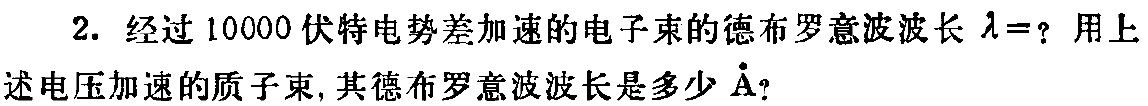
\includegraphics[width=\linewidth]{figures/2}
  \label{fig:}
\end{figure}

\begin{equation*}
  \begin{aligned}
    v = \sqrt{\dfrac{2 E_k}{m_0} } = 5.93097 \times 10^7 \  \mathrm{m/s}
  \end{aligned}
\end{equation*}
\begin{equation*}
  \begin{aligned}
    \lambda = \dfrac{h}{m_0 v} = 1.22643 \times 10^{-11} \  \mathrm{m} 
  \end{aligned}
\end{equation*}

\begin{figure}[H]
  \centering
  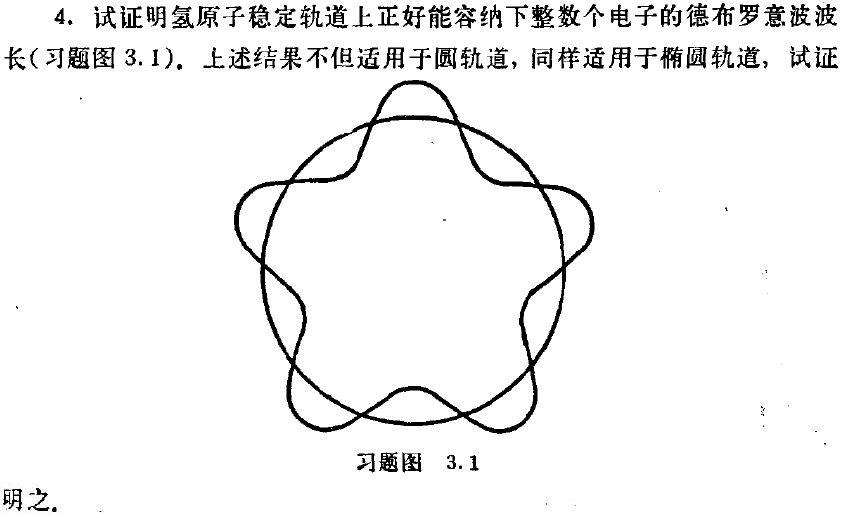
\includegraphics[width=\linewidth]{figures/4}
  \label{fig:}
\end{figure}

In round orbits

\begin{equation*}
  \begin{aligned}
    \oint p_r \md q_r = n_r h \\
    \oint p_\phi \md q_\phi = n_\phi h
  \end{aligned}
\end{equation*}

Since $p_r = 0$

\begin{equation*}
  \begin{aligned}
    \oint m r^2 \dot{\phi} \md \phi = n_\phi h
  \end{aligned}
\end{equation*}
\begin{equation*}
  \begin{aligned}
    2 \pi m v r = n_{\phi} h
  \end{aligned}
\end{equation*}

\begin{equation*}
  \begin{aligned}
    2 \pi r = n_{\phi} \dfrac{h}{m v} 
  \end{aligned}
\end{equation*}

The wave length of the electron is

\begin{equation*}
  \begin{aligned}
    \lambda = \dfrac{h}{p} = \dfrac{h}{m v}  
  \end{aligned}
\end{equation*}

So that

\begin{equation*}
  \begin{aligned}
    2 \pi r = n_{\phi} \lambda
  \end{aligned}
\end{equation*}

When the orbit is shaped in eclipse

\begin{equation*}
  \begin{aligned}
    \oint p_r \md q_r = n_r h \\
    \oint p_\phi \md q_\phi = n_\phi h
  \end{aligned}
\end{equation*}

So that

\begin{equation*}
  \begin{aligned}
    \oint \left( p_r \md r + p_{\phi} \md \phi \right) = n h
  \end{aligned}
\end{equation*}

\begin{equation*}
  \begin{aligned}
    \oint \left( m \dot{r} \md r + m r^2 \dot{\phi} \md \phi \right) = n h
  \end{aligned}
\end{equation*}

\begin{equation*}
  \begin{aligned}
    \oint \left( m \dot{r}^2 \md t + m r^2 \dot{\phi}^2 \md t \right) = n h
  \end{aligned}
\end{equation*}

\begin{equation*}
  \begin{aligned}
    \oint \left[ m \left( \dot{r}^2 + m r^2 \dot{\phi}^2 \right) \right] \md t = n h
  \end{aligned}
\end{equation*}

\begin{equation*}
  \begin{aligned}
    \oint \left[ m v^2 \right] \md t = n h
  \end{aligned}
\end{equation*}

\begin{equation*}
  \begin{aligned}
    \oint m v \md s = n h
  \end{aligned}
\end{equation*}

\begin{equation*}
  \begin{aligned}
    \oint \dfrac{m v}{h}  \md s = n
  \end{aligned}
\end{equation*}

The wavelength of the electron is

\begin{equation*}
  \begin{aligned}
    \lambda = \dfrac{h}{p} = \dfrac{h}{m v}  
  \end{aligned}
\end{equation*}

insert it into

\begin{equation*}
  \begin{aligned}
    \oint \dfrac{\md s}{\lambda}  = n
  \end{aligned}
\end{equation*}

\begin{equation*}
  \begin{aligned}
    \oint \md s = n \lambda
  \end{aligned}
\end{equation*}

\begin{figure}[H]
  \centering
  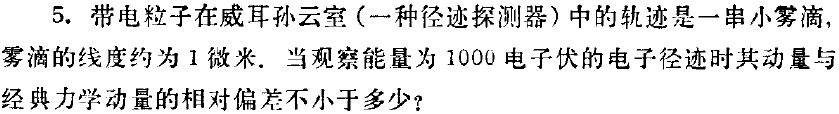
\includegraphics[width=\linewidth]{figures/5}
  \label{fig:}
\end{figure}

\begin{equation*}
  \begin{aligned}
    \Delta p \Delta x \ge \dfrac{\hbar}{2} 
  \end{aligned}
\end{equation*}

\begin{equation*}
  \begin{aligned}
    p = \sqrt{2 m E_k} 
  \end{aligned}
\end{equation*}

\begin{equation*}
  \begin{aligned}
    \dfrac{\Delta p}{p}  = \dfrac{\hbar}{2 \Delta x \sqrt{2 m E_k}} = 3.046 \times 10^{-5}
  \end{aligned}
\end{equation*}

\begin{figure}[H]
  \centering
  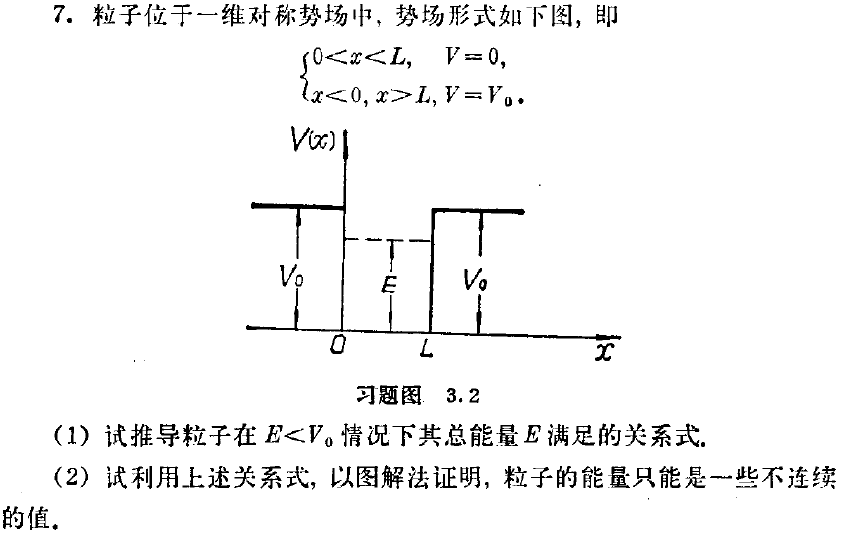
\includegraphics[width=\linewidth]{figures/7}
  \label{fig:}
\end{figure}
\begin{figure}[H]
  \centering
  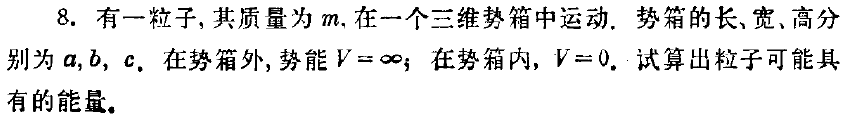
\includegraphics[width=\linewidth]{figures/8}
  \label{fig:}
\end{figure}

\end{document}